\documentclass[aspectratio=169]{beamer}

\usepackage{calc}
\usepackage{graphicx}
\usepackage{siunitx}
\usepackage{xcolor}

\graphicspath{{./images}}
\setbeamertemplate{navigation symbols}{}

\author{Chris Doble}
\date{}
\subtitle{Building a GPS receiver from scratch}
\title{Part 3: GPS signals}
\usetheme{Madrid}

% Show the topics frame at the start of each section
\AtBeginSection[]
{
  \begin{frame}
    \frametitle{Topics}
    \tableofcontents[currentsection]
  \end{frame}
}

\begin{document}

\frame{\titlepage}

\begin{frame}
    \frametitle{Topics}

    \tableofcontents
\end{frame}

\section{The C/A signal}

\begin{frame}
    \frametitle{GPS frequencies}

    \centering
    \only<1>{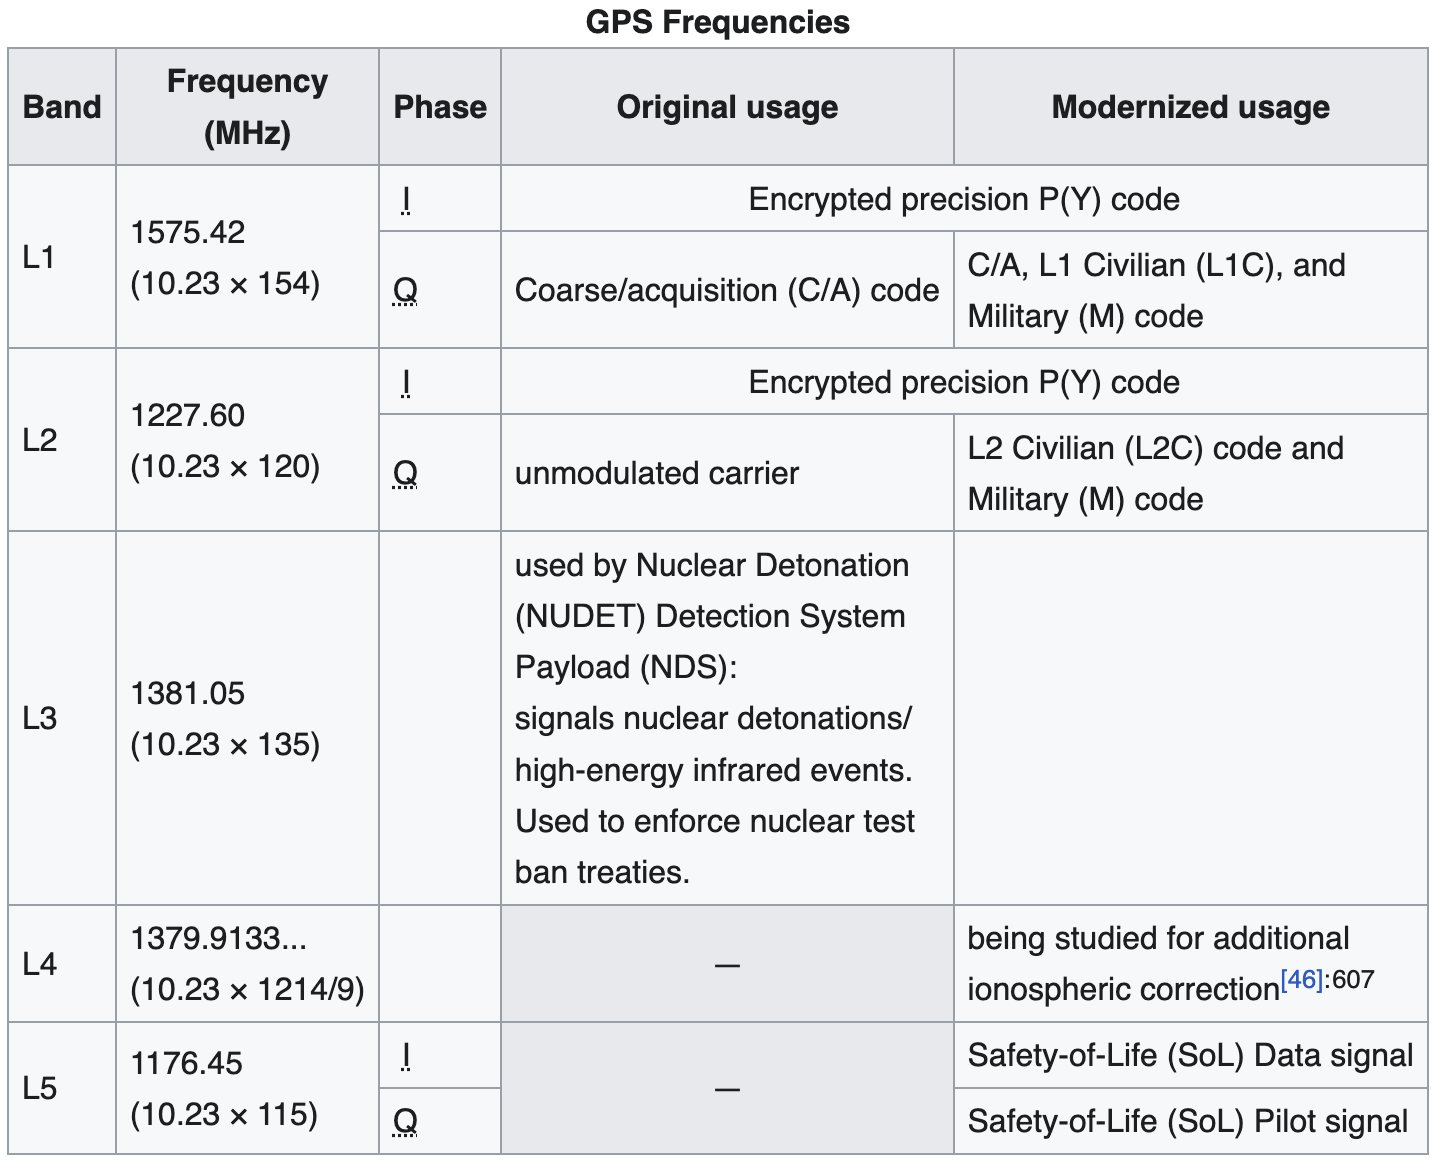
\includegraphics[width=\textwidth / 2]{1 gps frequencies.png}}%
    \only<2>{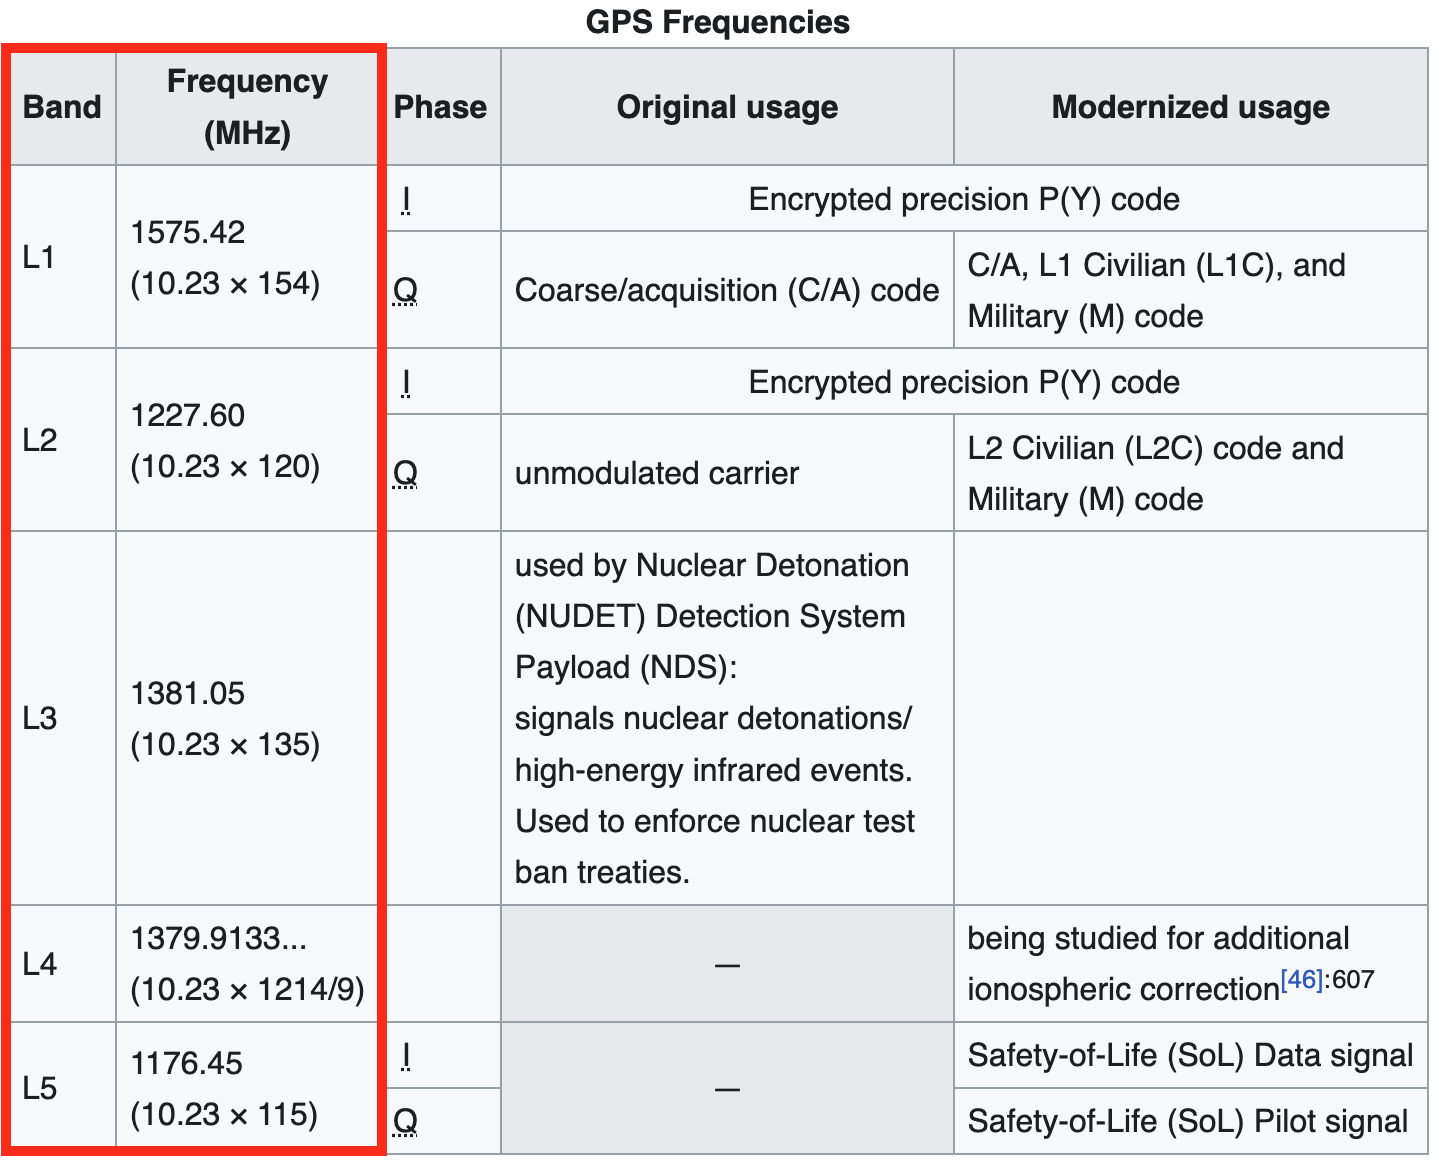
\includegraphics[width=\textwidth / 2]{2 gps frequencies.png}}%
    \only<3>{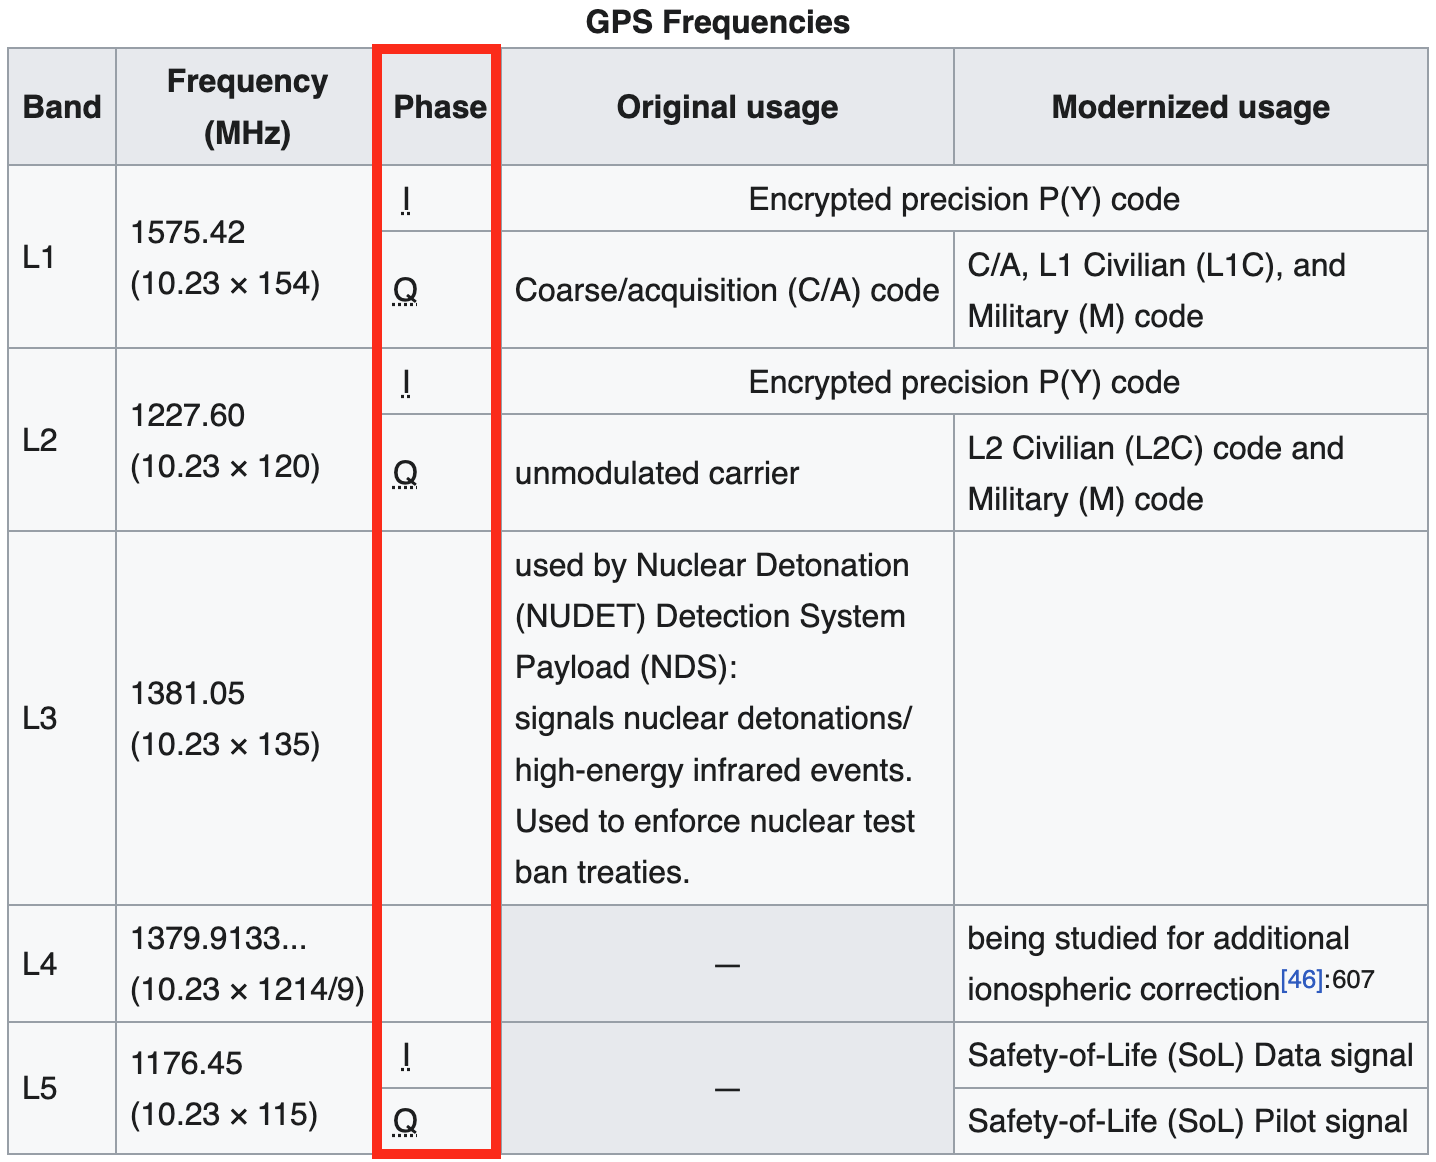
\includegraphics[width=\textwidth / 2]{3 gps frequencies.png}}%
    \only<4>{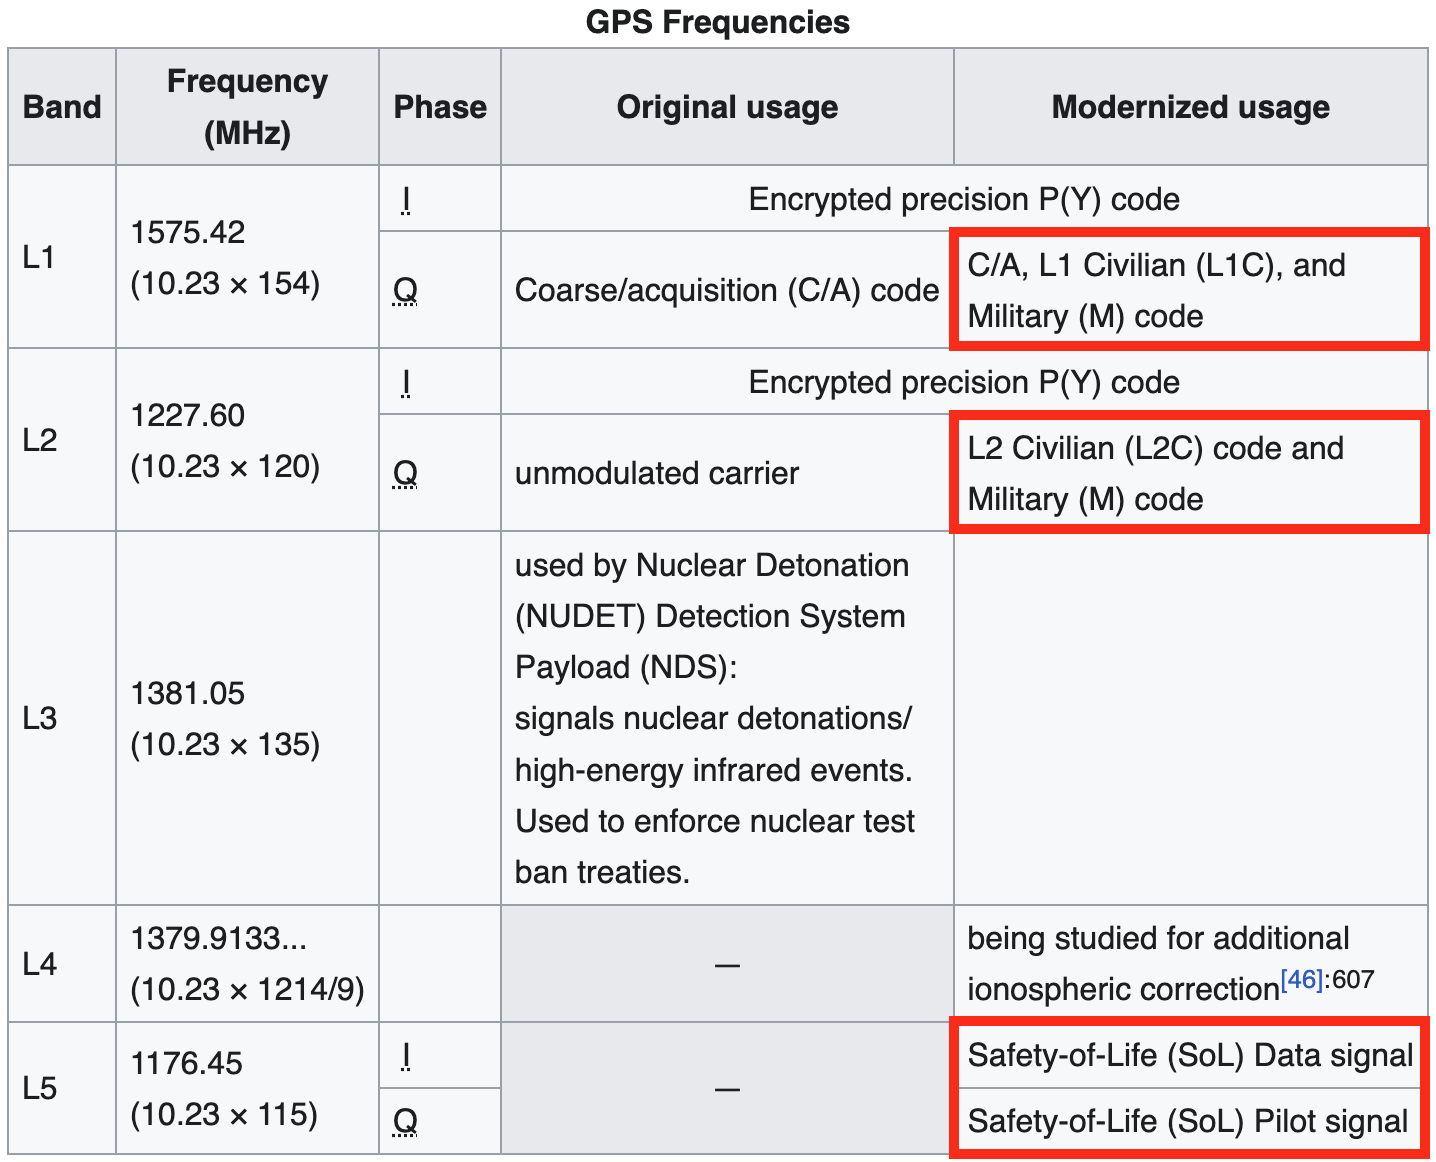
\includegraphics[width=\textwidth / 2]{4 gps frequencies.png}}%
    \only<5>{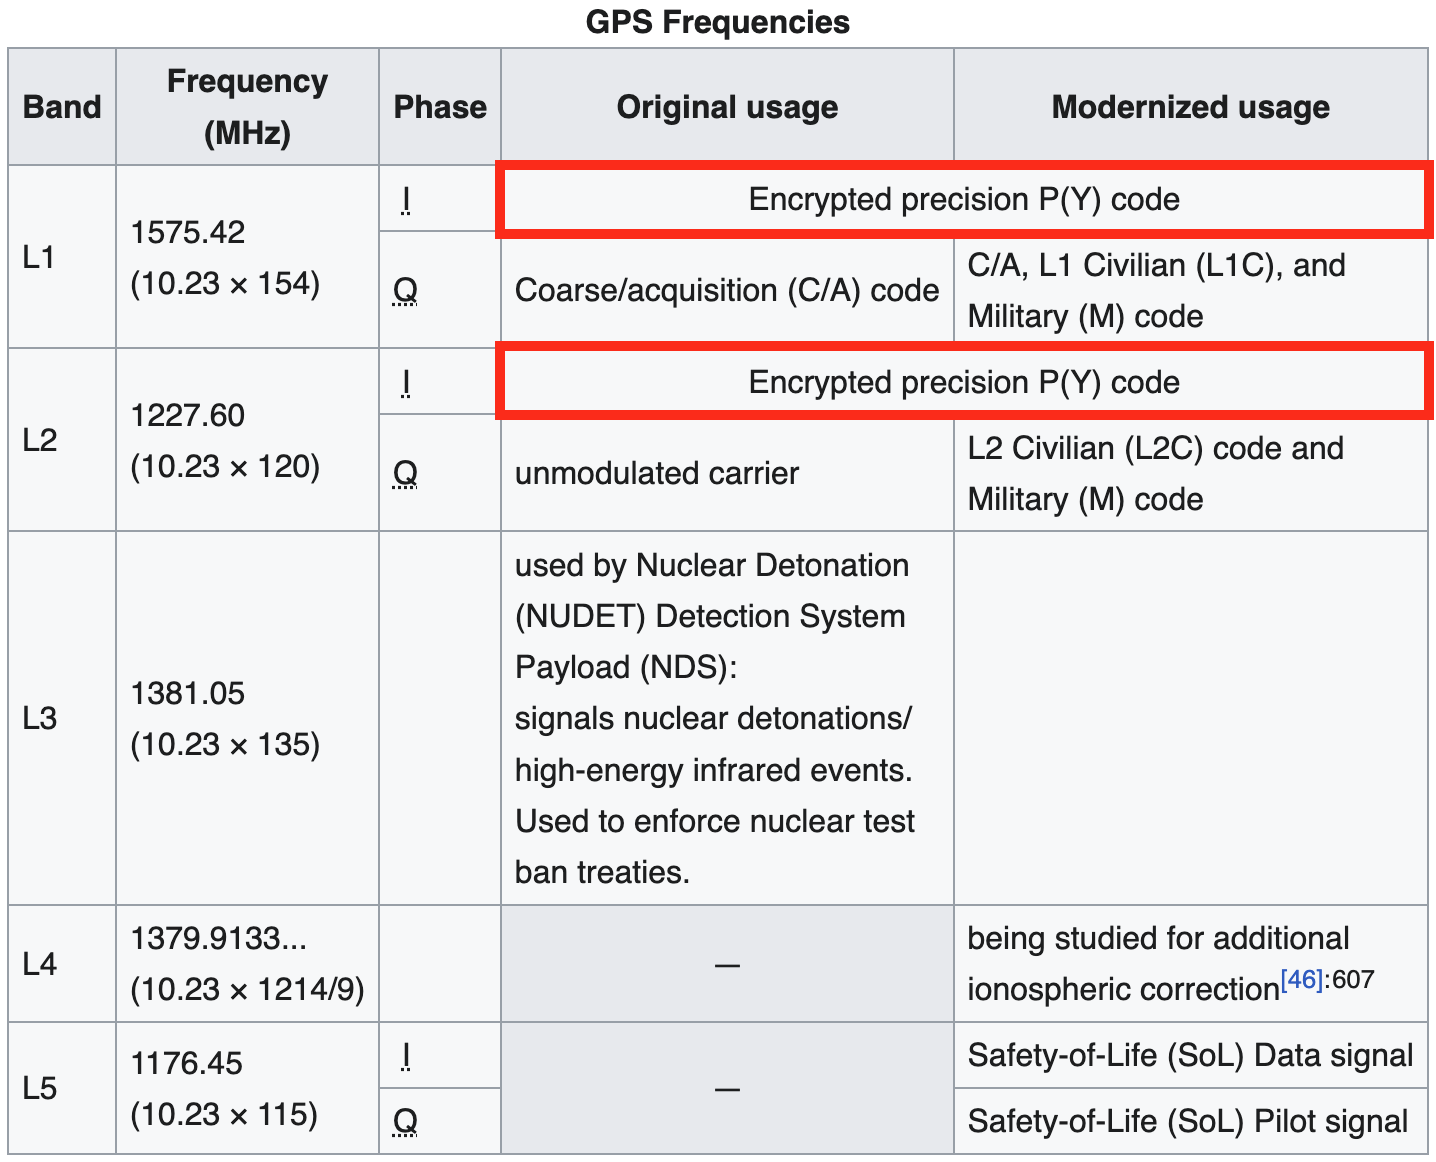
\includegraphics[width=\textwidth / 2]{5 gps frequencies.png}}%
    \only<6>{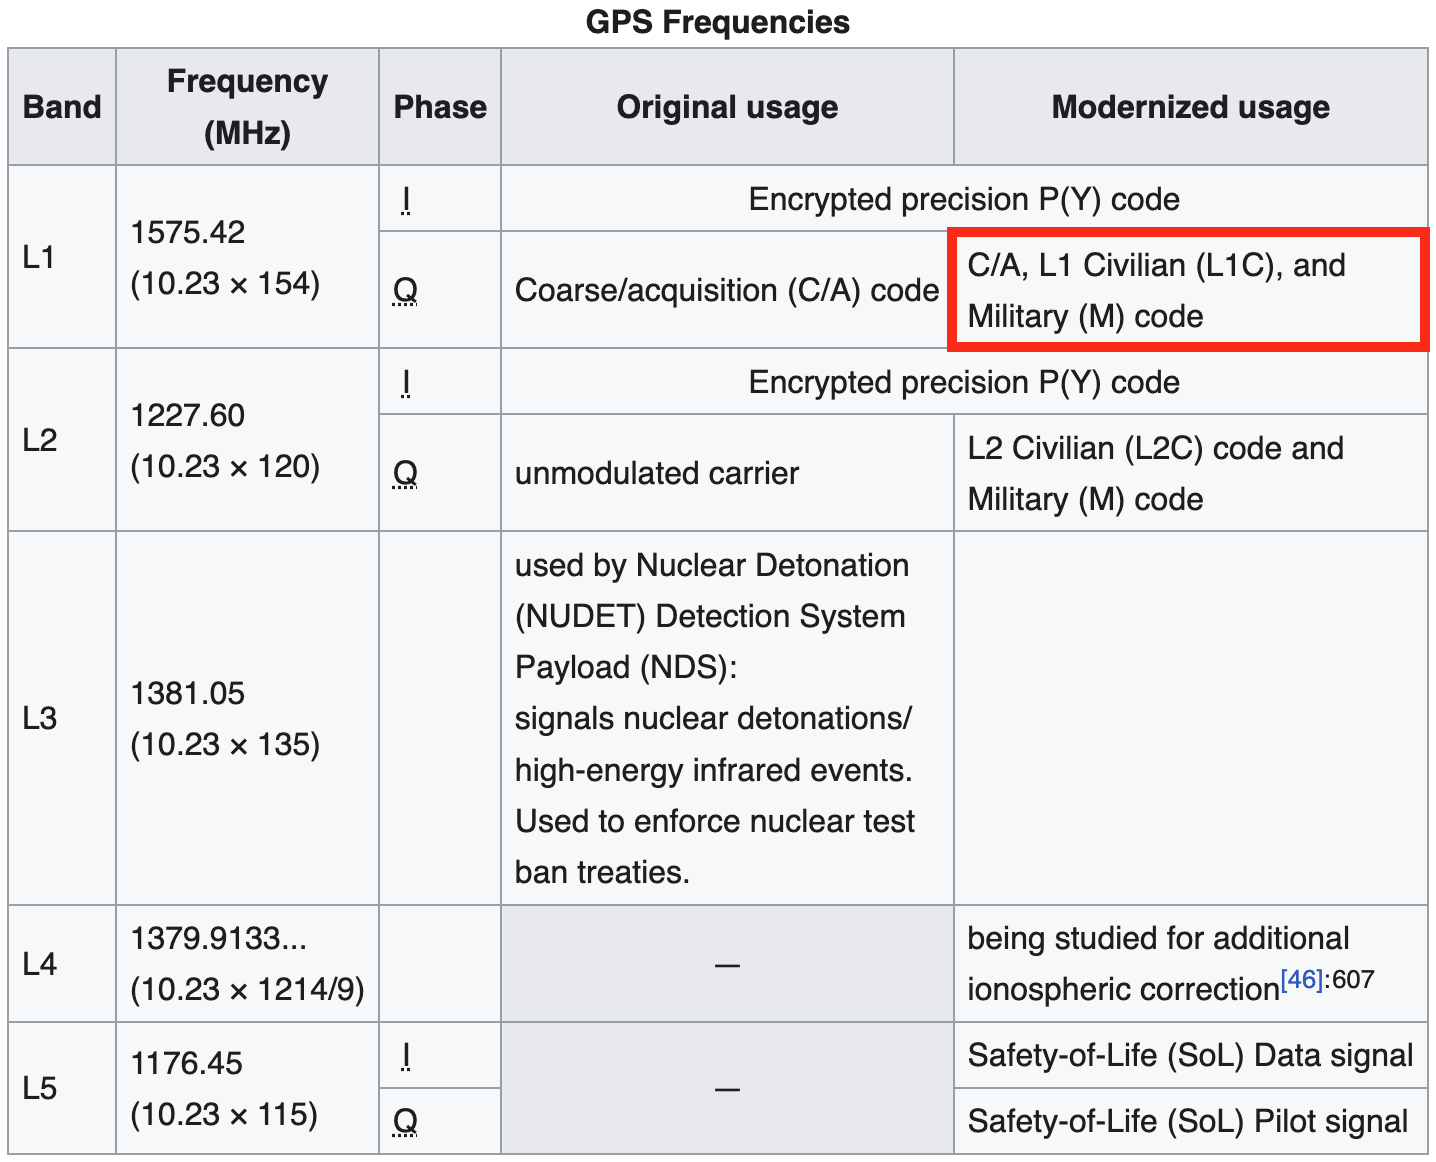
\includegraphics[width=\textwidth / 2]{6 gps frequencies.png}}%
    \\
    \texttt{\tiny{Source: "GPS signals" from Wikipedia, CC BY-SA 4.0, https://en.wikipedia.org/wiki/GPS\_signals}}
\end{frame}

\begin{frame}
    \frametitle{The navigation message}

    \begin{itemize}
        \item<2-> Binary
        
        \item<3-> Transmitted at 50 bps
        
        \item<4-> Contains the information required to calculate satellite location and time
        
        \item<5-> $D_i(t)$ represents the navigation message bit of satellite number $i$ at time $t$
    \end{itemize}
\end{frame}

\section{Modulation}

\begin{frame}
  \frametitle{Modulation}

  \centering
  \begin{tabular}{c c}
    \onslide<2->{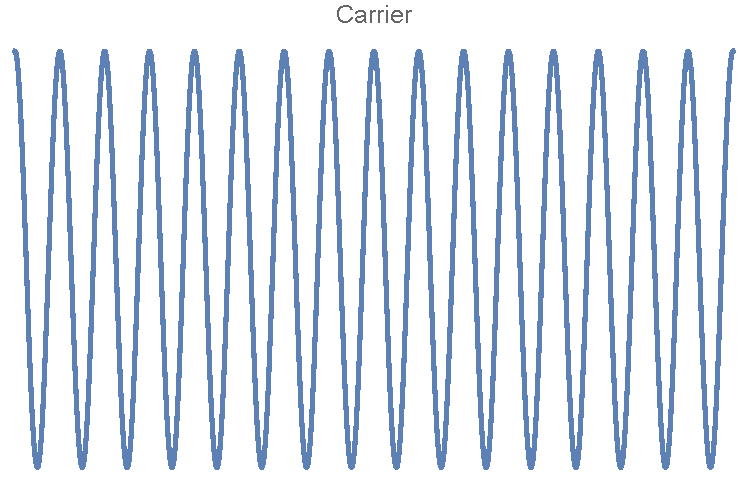
\includegraphics[width=\textwidth / 3]{7 carrier.pdf}} & \onslide<3->{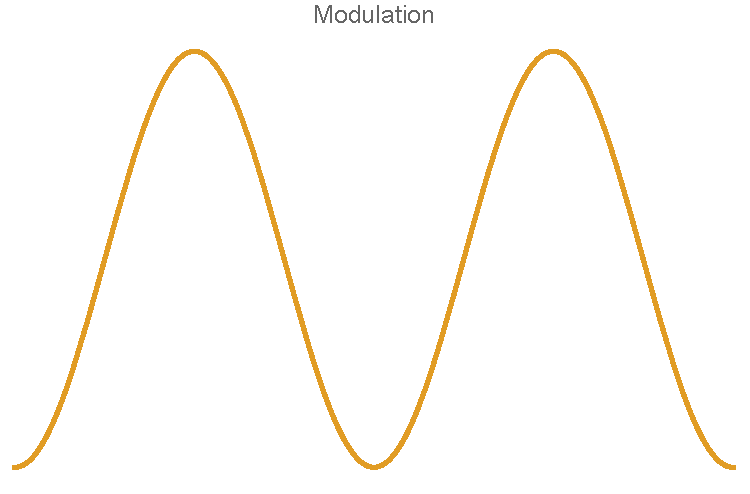
\includegraphics[width=\textwidth / 3]{8 modulation.pdf}} \\
    \onslide<4->{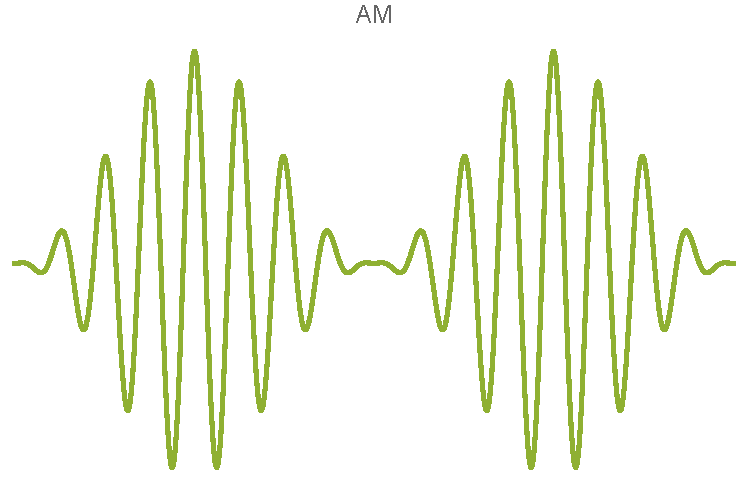
\includegraphics[width=\textwidth / 3]{9 am.pdf}}      & \onslide<5->{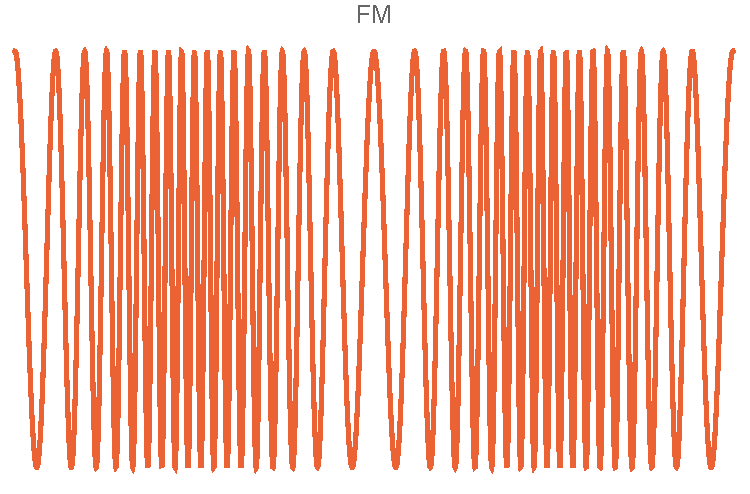
\includegraphics[width=\textwidth / 3]{10 fm.pdf}}
  \end{tabular}
\end{frame}

\begin{frame}
  \frametitle{Modulation of the C/A signal}

  \begin{itemize}
    \item<2-> The carrier signal is a radio wave at the L1 frequency, $\qty{1575.42}{MHz}$
    
    \item<3-> $f_i(t)$ is the amplitude of satellite number $i$'s carrier wave at time $t$
    
    \item<4-> The modulation signal is the navigation message $D_i(t)$, transmitted at $\qty{50}{bps}$
  \end{itemize}

  \leavevmode \\

  \centering
  \onslide<5->{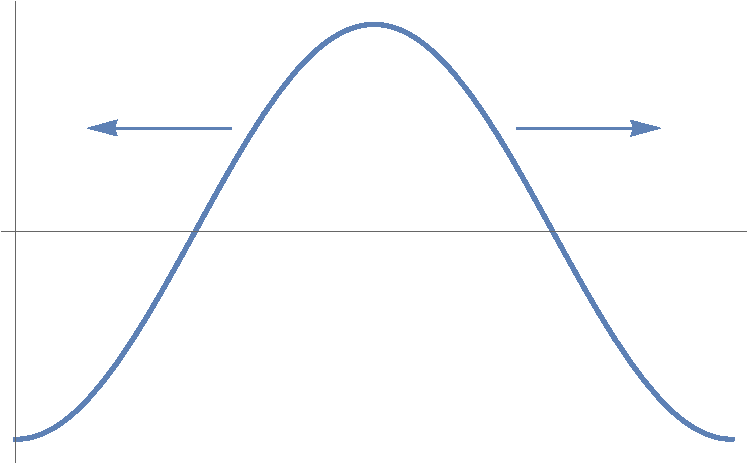
\includegraphics[width=\textwidth / 3]{11 phase shift.pdf}}
\end{frame}

\begin{frame}
  \frametitle{Modulation of the C/A signal}

  \begin{center}
    \huge
    \begin{tabular}{c c c c c c c}
      \onslide<1->{$D_i =$ & 0 & 1 & 0 & 0 & 1 & 1 \\}
      & \onslide<2>{$\downarrow$} & \onslide<3>{$\downarrow$} & \onslide<2>{$\downarrow$} & \onslide<2>{$\downarrow$} & \onslide<3>{$\downarrow$} & \onslide<3>{$\downarrow$} \\
      \onslide<4->{$\hat{D}_i =$} & \onslide<2->{1} & \onslide<3->{-1} & \onslide<2->{1} & \onslide<2->{1} & \onslide<3->{-1} & \onslide<3->{-1} \\
    \end{tabular}

    \leavevmode \newline

    \onslide<5->{$\hat{D}_i(t) f_i(t)$}
  \end{center}
\end{frame}

\section{CDMA}

\begin{frame}
  \frametitle{PRN codes}

  \begin{itemize}
    \item<2-> Each satellite is assigned a pseudorandom noise code (PRN code)
    
    \begin{itemize}
      \item<3-> Binary
      
      \item<4-> 1023 bits long
    \end{itemize}
  \end{itemize}

  \leavevmode \newline

  \onslide<5->{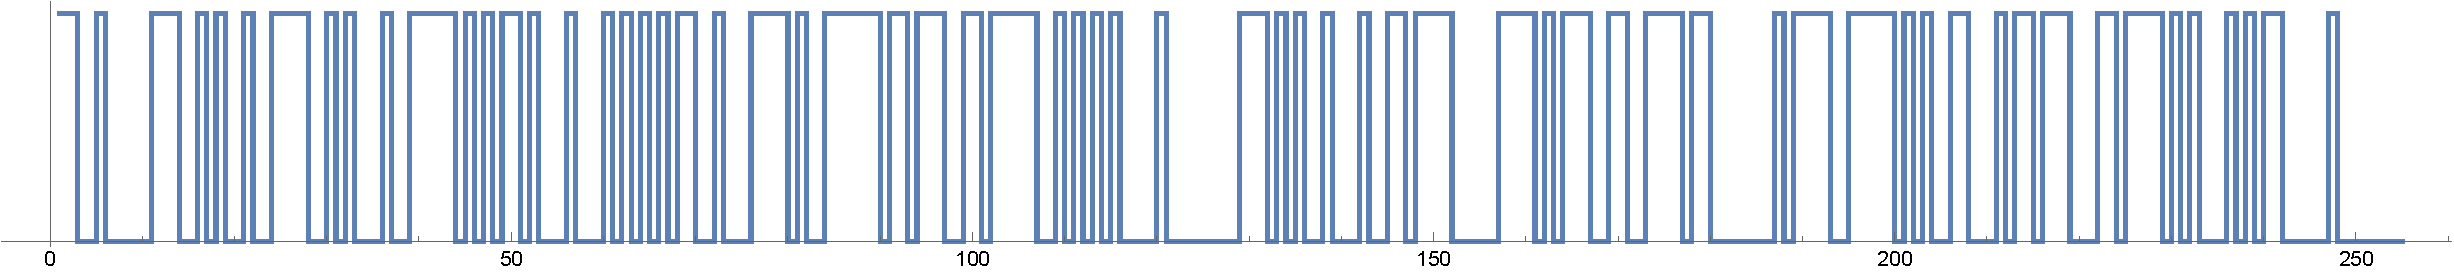
\includegraphics[width=\textwidth]{12 prn code.pdf}}
\end{frame}

\begin{frame}
  \frametitle{PRN codes}

  \begin{itemize}
    \item<2-> Satellites modulate $D_i(t) \oplus PRN_i(t)$
    
    \item<3-> $PRN_i(t)$ is the bit of satellite number $i$'s PRN code at time $t$
    
    \item<4-> Transmitted at $\qty{1.023}{Mbps}$
      
    \item<4-> Full code repeats once per millisecond, 20 times per navigation message bit
  \end{itemize}

  \onslide<5->{
    \begin{center}
      $0 \rightarrow 1$, $1 \rightarrow -1$

      \vspace{1em}

      \begin{tabular}{c c}
        \begin{tabular}{|c|c|c|}
          \hline
          $\oplus$ & 0 & 1 \\
          \hline
          0 & 0 & 1 \\
          \hline
          1 & 1 & 0 \\
          \hline
        \end{tabular}

        \begin{tabular}{|c|c|c|}
          \hline
          $\times$ & 1 & -1 \\
          \hline
          1 & 1 & -1 \\
          \hline
          -1 & -1 & 1 \\
          \hline
        \end{tabular}
      \end{tabular}
    \end{center}
  }

  \begin{itemize}
    \item<6-> The signal transmitted by a satellite is $\hat{D}_i(t) \hat{PRN}_i(t) f_i(t)$
  \end{itemize}
\end{frame}

\begin{frame}
  \frametitle{The properties of PRN codes}

  \begin{itemize}
    \item<2-> Strong, positive correlation with an aligned version of itself
    
    \item<3-> Near-zero correlation with misaligned versions of itself
  \end{itemize}

  \vspace{0.5em}

  \centering
  \onslide<4->{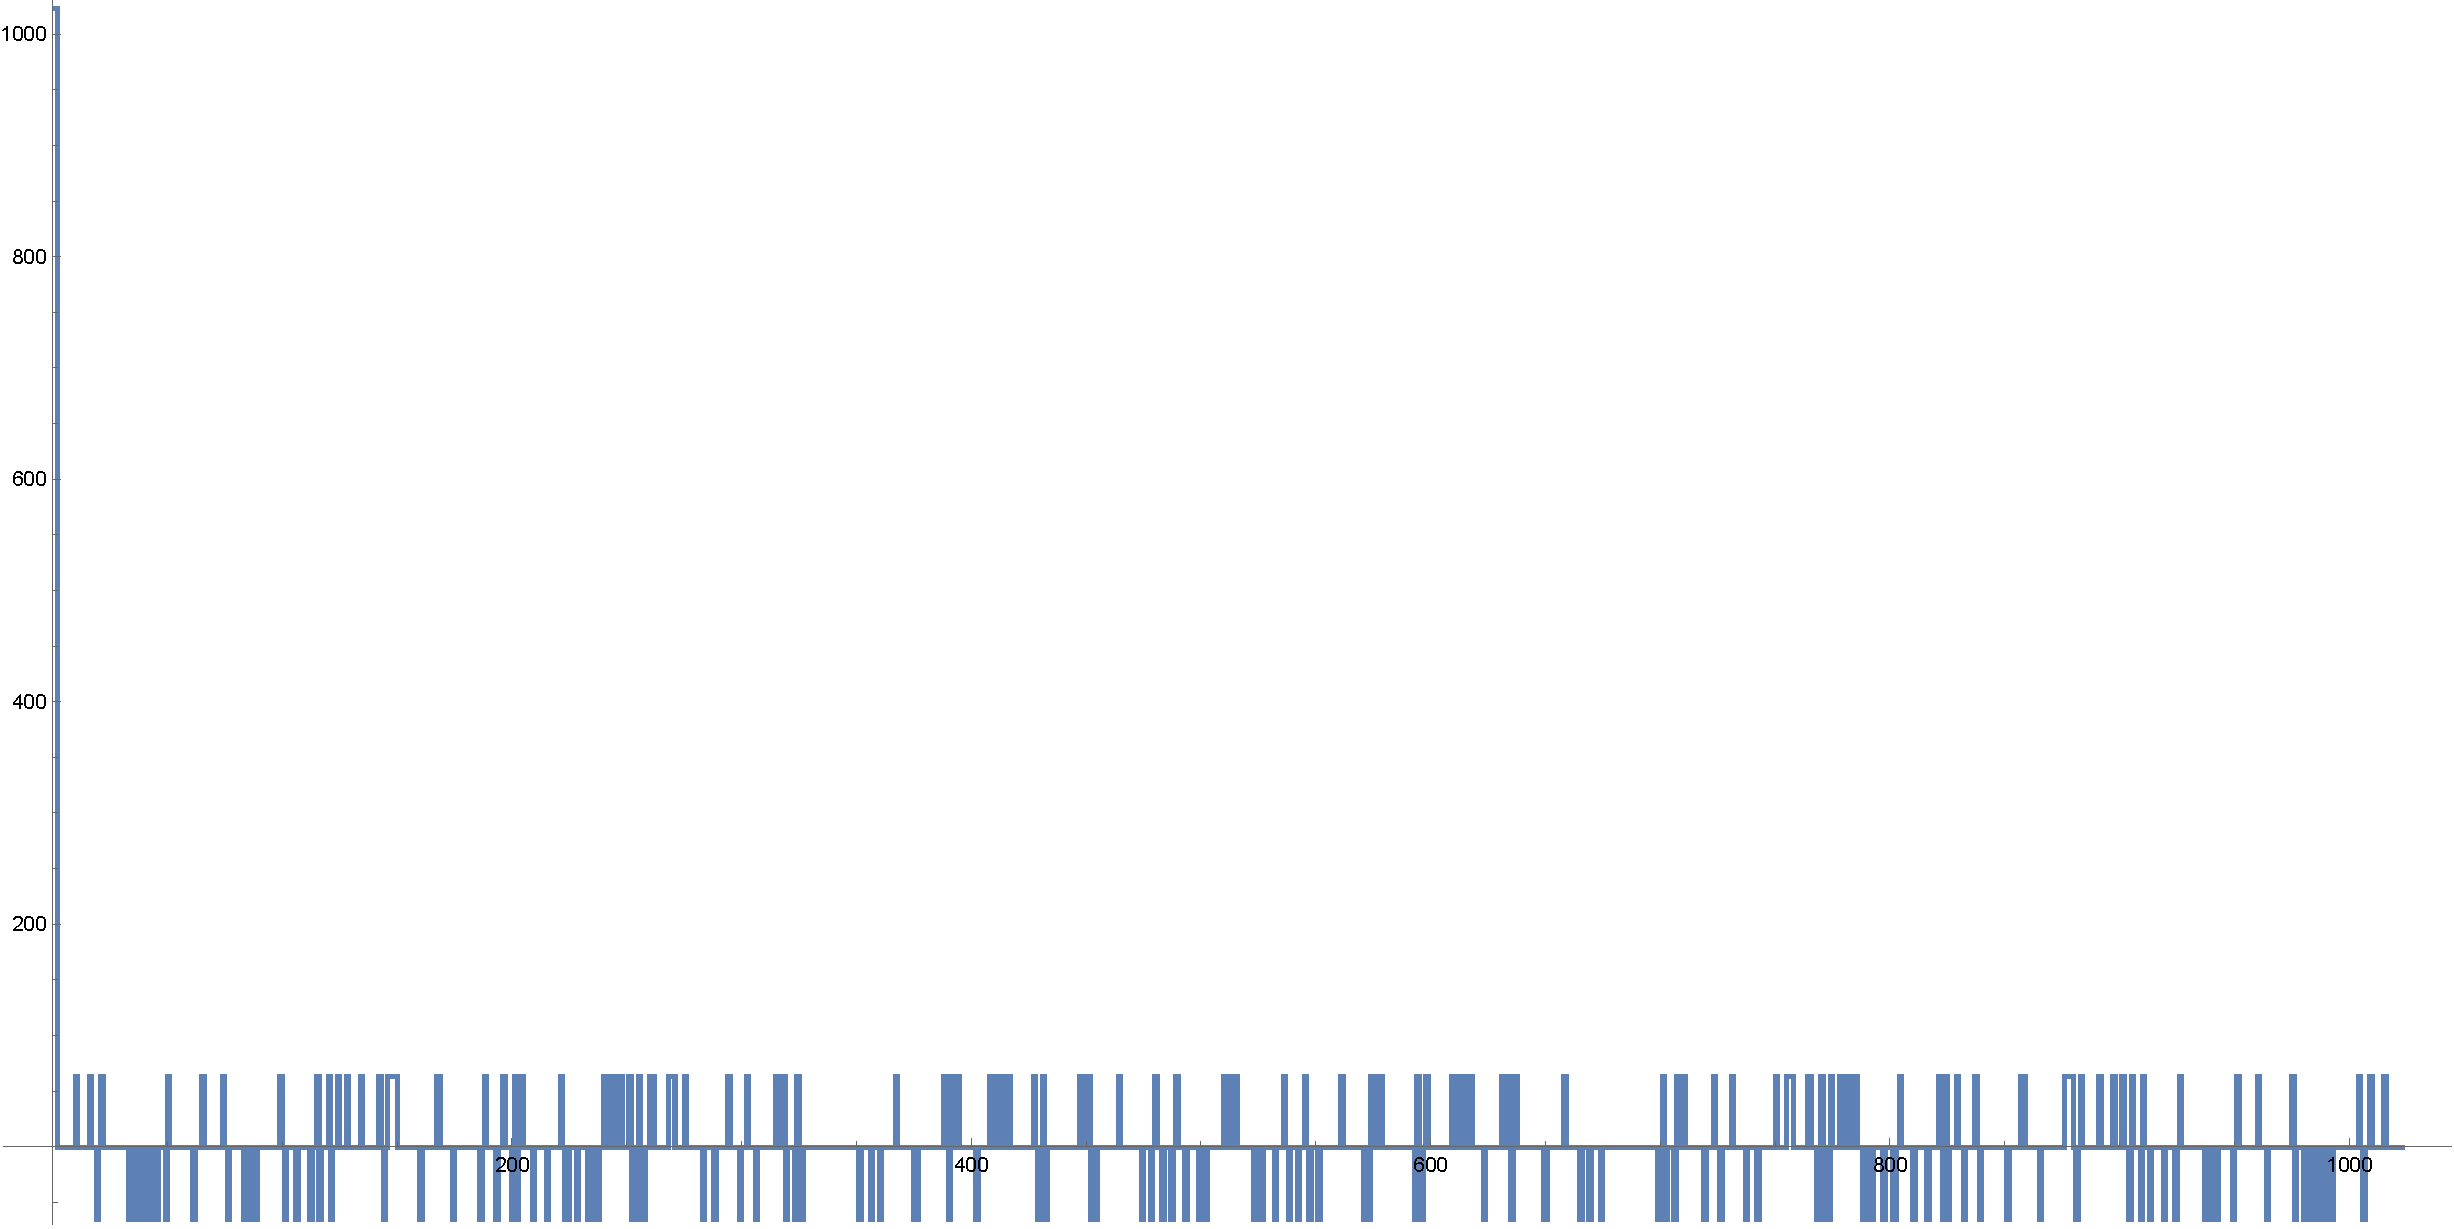
\includegraphics[width=\textwidth * 3 / 4]{13 autocorrelation.pdf}}
\end{frame}

\begin{frame}
  \frametitle{The properties of PRN codes}

  \begin{itemize}
    \item<2-> The correlation of two different PRN codes is always near zero
  \end{itemize}

  \vspace{0.5em}

  \centering
  \onslide<3->{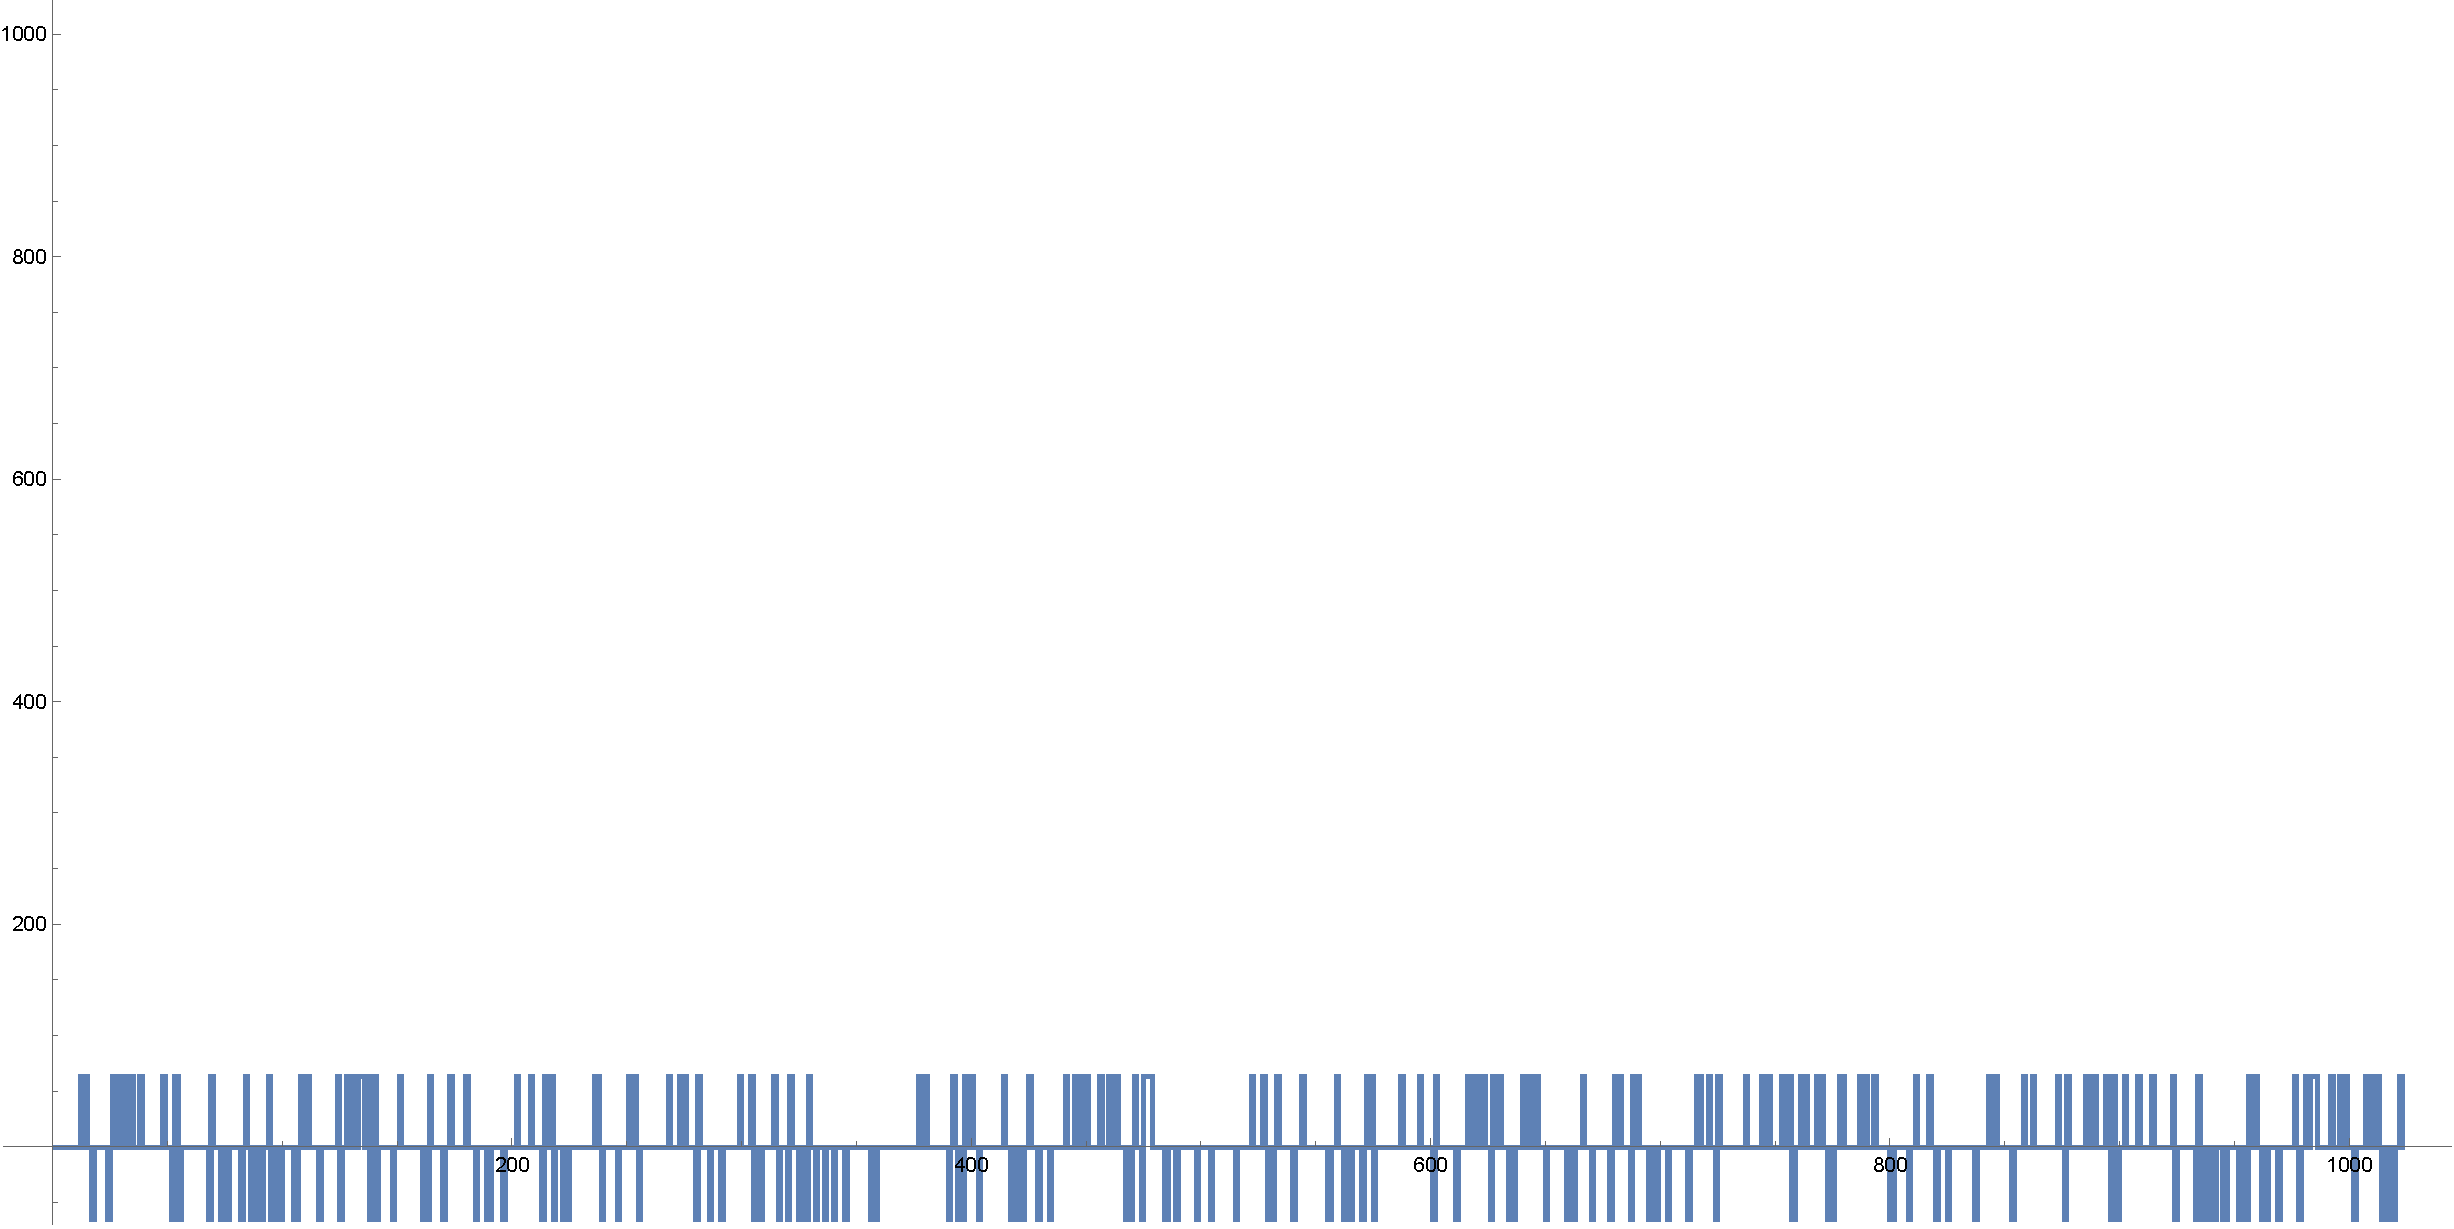
\includegraphics[width=\textwidth * 3 / 4]{14 cross-correlation.pdf}}
\end{frame}

\begin{frame}
  \frametitle{Decoding a bit from a satellite}

  \centering
  \Large

  \only<2>{\[\hat{D}_i(t) \hat{PRN}_i(t) f_i(t)\]}
  \only<3>{\[\hat{D}_1(t) \hat{PRN}_1(t) f_1(t) + \hat{D}_2(t) \hat{PRN}_2(t) f_2(t)\]}
  \only<4>{\[\hat{D}_1(t) \hat{PRN}_1(t) f_1(t) + \hat{D}_2(t) \hat{PRN}_2(t) f_2(t) + \textcolor{red}{N_1(t)}\]}
  \only<5>{\[\hat{D}_1(t) \hat{PRN}_1(t) \textcolor{red}{f_1(t)} + \hat{D}_2(t) \hat{PRN}_2(t) \textcolor{red}{f_2(t)} + N_1(t)\]}
  \only<6>{\[\textcolor{red}{c_1} \hat{D}_1(t) \hat{PRN}_1(t) + \textcolor{red}{c_2} \hat{D}_2(t) \hat{PRN}_2(t) + \textcolor{red}{N_2(t)}\]}
  \only<7>{\[\textcolor{red}{\int_0^T [} c_1 \hat{D}_1(t) \hat{PRN}_1(t) + c_2 \hat{D}_2(t) \hat{PRN}_2(t) + N_2(t) \textcolor{red}{] \hat{PRN}_1(t) \,dt}\]}
  \only<8>{\[\int_0^T [c_1 \hat{D}_1(t) \hat{PRN}_1(t) + c_2 \hat{D}_2(t) \hat{PRN}_2(t) + N_2(t)] \hat{PRN}_1(t \begingroup \color{red} - \tau \endgroup) \,dt\]}
  \only<9>{
    \begin{align*}
      & \int_0^T c_1 \hat{D}_1(t) \hat{PRN}_1(t) \hat{PRN}_1(t - \tau) \,d t \\
      & \qquad + \int_0^T c_2 \hat{D}_2(t) \hat{PRN}_2(t) \hat{PRN}_1(t - \tau) \,d t \\
      & \qquad + \int_0^T N_2(t) \hat{PRN}_1(t - \tau) \,d t
    \end{align*}
  }
  \only<10>{
    \begin{align*}
      & \textcolor{red}{c_1} \int_0^T \hat{D}_1(t) \hat{PRN}_1(t) \hat{PRN}_1(t - \tau) \,d t \\
      & \qquad + \textcolor{red}{c_2} \int_0^T \hat{D}_2(t) \hat{PRN}_2(t) \hat{PRN}_1(t - \tau) \,d t \\
      & \qquad + \int_0^T N_2(t) \hat{PRN}_1(t - \tau) \,d t
    \end{align*}
  }
  \only<11>{
    \begin{align*}
      & c_1 \textcolor{red}{\hat{D}_1(0)} \int_0^T \hat{PRN}_1(t) \hat{PRN}_1(t - \tau) \,d t \\
      & \qquad + c_2 \textcolor{red}{\hat{D}_2(0)} \int_0^T \hat{PRN}_2(t) \hat{PRN}_1(t - \tau) \,d t \\
      & \qquad + \int_0^T N_2(t) \hat{PRN}_1(t - \tau) \,d t
    \end{align*}
  }
  \only<12>{\[c_1 \hat{D}_1(0) \int_0^T \hat{PRN}_1(t) \hat{PRN}_1(t - \tau) \,d t + \int_0^T N_2(t) \hat{PRN}_1(t - \tau) \,d t\]}
  \only<13>{\[c_1 \hat{D}_1(0) \int_0^T \hat{PRN}_1(t) \hat{PRN}_1(t) \,d t + \int_0^T N_2(t) \hat{PRN}_1(t) \,d t\]}
  \only<14>{\[\textcolor{red}{\alpha} \hat{D}_1(0) + \int_0^T N_2(t) \hat{PRN}_1(t) \,d t\]}
  \only<15>{\[\alpha \hat{D}_1(0) + \textcolor{red}{\beta}\]}
\end{frame}

\begin{frame}
  \frametitle{Recap}

  \begin{itemize}
    \item<2-> We'll use the C/A signal on the L1 frequency
    
    \item<3-> The C/A signal contains the navigation message
    
    \item<4-> The navigation message lets us calculate a satellite's location and time
    
    \item<5-> Each satellite is assigned a PRN code
    
    \item<6-> The PRN code is XOR-ed with the navigation message and repeats once per ms
    
    \item<7-> To decode the navigation message bit of satellite number $i$:
    
    \begin{itemize}
      \item<8-> Record the received signal for $\qty{1}{ms}$
      
      \item<9-> Calculate its correlation with an aligned copy of satellite number $i$'s PRN code
    \end{itemize}
  \end{itemize}
\end{frame}

\end{document}